\documentclass[12pt,a4paper]{article}
\usepackage[14pt]{extsizes}
\usepackage[utf8]{inputenc}
\usepackage{amsmath}
\usepackage{amsfonts}
\usepackage{amssymb}
\usepackage{tabularx}
\usepackage{multirow}
\newcommand{\RomanNumeralCaps}[1]
{\MakeUppercase{\romannumeral #1}}
\usepackage{cmap} % для кодировки шрифтов в pdf
\usepackage[T2A]{fontenc}
\usepackage[russian]{babel}
\usepackage{graphicx} % для вставки картинок
\usepackage{amssymb,amsfonts,amsmath,amsthm} % математические дополнения от АМС
\usepackage{indentfirst} % отделять первую строку раздела абзацным отступом тоже
\usepackage[outdir=./]{epstopdf}
\usepackage{listings}
\usepackage{color} %red, green, blue, yellow, cyan, magenta, black, white
\definecolor{mygreen}{RGB}{28,172,0} % color values Red, Green, Blue
\definecolor{mylilas}{RGB}{170,55,241}
% Поля
\usepackage{geometry}
\geometry{left=2.5cm}
\geometry{right=1.5cm}
\geometry{top=1.5cm}
\geometry{bottom=2cm}

%%%%%%%%%%%%%%%%%%%%%%%%%%%%%%%    

\linespread{1.5} % полуторный интервал
\renewcommand{\rmdefault}{ftm} % Times New Roman
%\renewcommand{\rmdefault}{PT-Astra-Serif_Regular}
%\usefont{T2A}{PT-Astra-Serif_Regular}{m}{it}
\frenchspacing

% подключаем hyperref (для ссылок внутри  pdf)
\usepackage[unicode, pdftex]{hyperref}

% коррекция подрисуночной подписи
\usepackage{caption}
\captionsetup[figure]{labelsep=period} %Точка
%\captionsetup[figure]{labelsep=space}  %Пробел
%\captionsetup[figure]{labelsep=endash}  %Новый страндарт
\usepackage[figurename=Рисунок]{caption}
\usepackage{longtable}


\begin{document}
	
	\begin{titlepage}
		
		\begin{center}
			САНКТ-ПЕТЕРБУРГСКИЙ ГОСУДАРСТВЕННЫЙ ЭЛЕКТРОТЕХНИЧЕСКИЙ УНИВЕРСИТЕТ «ЛЭТИ» ИМ. В.И. УЛЬЯНОВА (ЛЕНИНА)\\
			\vspace{0.1cm}
			Кафедра теоретических основ электротехники\\
			
			
			
		\end{center}
		
		\vspace{5cm}
		\begin{center}
			\begin{large}
				Лабораторная работа 5 \\
				"Метод Ньютона"
			\end{large}
		\end{center}
		
		\vspace{5cm}
		
		\hspace{5cm} Студент гр.  0307 \hrulefill Латин Я.М.
		
		\vspace{0.5cm}
		\hspace{5cm} Преподаватель \hrulefill Солнышкин С.Н. \\
		
		
		\vfill
		\begin{center}
			Санкт-Петербург\\
			2022
		\end{center}
		
		
	\end{titlepage}
\tableofcontents
\newpage

\section{Задание}
\subsection{Численно решить методом Ньютона уравнение }
\begin{equation*}
 7.8x^2 -3.1x-2.4=2.1\sin(4.7x-3.2)
 \end{equation*}
\subsection{Численно решить методом Ньютона систему уравнений}
\begin{equation*}
	\begin{cases}
		4e^{-0.8y}-3x=9e^{0.7x}-2y-5
		\\
		6x^4+7y^6=881-229x-775y
	\end{cases}	
\end{equation*}

\section{Решение уравнения}
Уравнение в стандартной форме:
\begin{equation*}
	f(x)=0 , \text{  ~где~ } f(x)=4e^{-0.8y}-3x-9e^{0.7x}+2y+5
\end{equation*}


Производная: 
\begin{equation*}
	f'(x)=-\dfrac{987\cos\left(\frac{47x}{10}-\frac{16}{5}\right)-1560x+310}{100}
\end{equation*}

Полученные значения уравнений:\\
$x_1=-0.51641140973316$\\
$x_2=0.9817349514171161$
\newpage
\begin{flushright}
	Таблица 1. Первый корень.
\end{flushright}
\begin{table}[!h]
	\centering
	\begin{tabular}{|c|c|c|}
		\hline
		k & $x_k$               & $f(x_k)$              \\ \hline
		0 & -0.5                & -0.3054037002801488   \\ \hline
		1 & -0.5167492544118317 & 0.006413807394519244  \\ \hline
		2 & -0.5164115415239419 & 2.501003745436492e-06 \\ \hline
		3 & -0.5164114097331801 & 3.810285420513537e-13 \\ \hline
		4 & -0.51641140973316   & 0                     \\ \hline
		5 & -0.51641140973316   & 0                     \\ \hline
	\end{tabular}
\end{table}
\begin{flushright}
	Таблица 2. Второй корень.
\end{flushright}

\begin{table}[!h]
	\centering
	\begin{tabular}{|c|c|c|}
		\hline
		k & $x_k$              & $f(x_k)$               \\ \hline
		0 & 1                  & 0.2052605281314848     \\ \hline
		1 & 0.9826077281554022 & 0.009340570687955463   \\ \hline
		2 & 0.9817371325150148 & 2.32840705227666e-05   \\ \hline
		3 & 0.9817349514308014 & 1.460960241672637e-10  \\ \hline
		4 & 0.981734951417116  & -1.332267629550188e-15 \\ \hline
		5 & 0.9817349514171161 & 4.440892098500626e-16  \\ \hline
		6 & 0.9817349514171161 & 4.440892098500626e-16  \\ \hline
	\end{tabular}

\end{table}
\newpage
	\begin{figure}[h!] 
	\centering
	\renewcommand{\figurename}{Рисунок}
	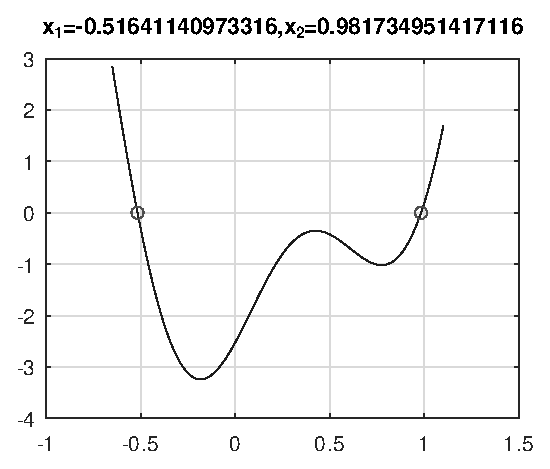
\includegraphics [width=0.65\textwidth]{../equation.eps}\\ 
	\caption{График уравнения  \label{fig.1}}
\end{figure}

\section{Решение системы}
\begin{equation*}
	\begin{cases}
		f_1(x,y)=0
		\\
		f_2(x,y)=0
	\end{cases}
	\Leftrightarrow
	\vec{f}(\vec{r})=\vec{0},~
	\vec{r}^*=\lim_{k\to \infty}\vec{r}_k,~
	\vec{r}_{k+1}=\vec{r}_k-(\vec{f}'(\vec{r}_k))^{-1}\vec{f}(\vec{r}_k),~
\end{equation*}

\begin{equation*}
	\vec{f}(\vec{r})=
	\begin{pmatrix}
		f_1(x,y)
		\\
		f_2(x,y)
	\end{pmatrix}
=
\begin{pmatrix}
	4\exp(-0.8y)-3x-9\exp(0.7x)+2y+5\\
	6x^4+7y^6-881+229x+775y
\end{pmatrix}
\end{equation*}

\begin{equation*}
	\vec{f}(\vec{r})=
	\begin{pmatrix}
		(f_1(x,y))'_x & (f_1(x,y))'_y
		\\
		(f_2(x,y))'_x & (f_2(x,y))'_y
	\end{pmatrix}
	=
\end{equation*}
\begin{equation*}
	=
	\begin{pmatrix}
		\left( -\dfrac{63\exp{\left( \dfrac{7x}{10} \right)}}{10}-3 \right) & \left( 2-\dfrac{16\exp{\left( \dfrac{-4y}{5} \right)}}{5} \right)\\
		\left( 624x^3+229 \right) & \left( 42y^5+775 \right)
	\end{pmatrix}
\end{equation*}
\newpage
Полученные значения уравнений:\\
$\vec{r}^*_1=(-0.01352039310251973,1.122683354922814)$\\
$\vec{r}^*_2=(1.648549264084652,-2.668437851904707)$

\begin{flushright}
	Таблица 3. Первая пара корней.
\end{flushright}
\begin{table}[h]
	\begin{flushleft}
		\begin{tabular}{|c|c|c|c|c|}
			\hline
			k & $x_k$                & $y_k$             & $f_1(x_k,y_k)$         & $f_2(x_k,y_k)$        \\ \hline
			0 & 0                    & 1.1               & -0.1408683532736745    & -16.09907299999986    \\ \hline
			1 & -0.013499810094  & 1.12277425374  & -0.0001268803060 & 0.081970636395226   \\ \hline
			2 & -0.013520393341 & 1.122683356609 & 3.3821372369402e-09  & 1.378521346850e-06 \\ \hline
			3 & -0.013520393102 & 1.122683354922 & -1.7763568394e-15  & -1.136868377216e-13 \\ \hline
			4 & -0.013520393102 & 1.122683354922 & 1.7763568394e-15   & 1.136868377216e-13  \\ \hline
		\end{tabular}
	\end{flushleft}
	
\end{table}

\begin{flushright}
	Таблица 3. Вторая пара корней.
\end{flushright}

\begin{table}[!h]
	\begin{tabular}{|c|c|c|c|c|}
		\hline
		k & $x_k$             & $y_k$              & \multicolumn{1}{c|}{$f_1(x_k,y_k)$} & \multicolumn{1}{c|}{$f_2(x_k,y_k)$} \\ \hline
		0 & 1.6               & -2.8               & 4.589637320134111     & 727.953727999999      \\ \hline
		1 & 1.66002753417 & -2.684153121745 & 0.13179360310917    & 82.32259370818     \\ \hline
		2 & 1.64874971524 & -2.668690117782 & 0.00171555298062  & 1.30577927845479     \\ \hline
		3 & 1.64854931841 & -2.668437917997 & 4.07641311817030e-07 & 0.0003426307775953 \\ \hline
		4 & 1.64854926408 & -2.668437851904 & 3.55271367880050e-14 & 2.41016095969e-11  \\ \hline
		5 & 1.64854926408 & -2.668437851904 & -1.1546319456101e-14& -1.364242052659e-12              \\ \hline
		6 & 1.64854926408 & -2.668437851904 & 1.77635683940025e-15  & 9.094947017729e-13 \\ \hline
		7 & 1.64854926408 & -2.668437851904 & 8.88178419700125e-15 & 4.547473508864e-13 \\ \hline
	\end{tabular}

\end{table}
\newpage
\begin{figure}[!h] 
	\centering
	\renewcommand{\figurename}{Рисунок}
	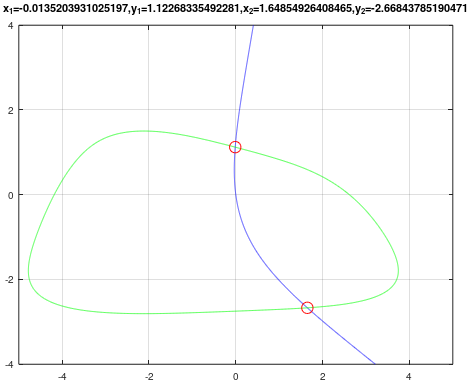
\includegraphics [width=0.65\textwidth]{../octave-gui_ro0Djm1Yqy.png}\\ 
	\caption{График системы  \label{fig.2}}
\end{figure}

\lstset{language=Matlab,%
	%basicstyle=\color{red},
	breaklines=true,%
	morekeywords={matlab2tikz},
	keywordstyle=\color{blue},%
	morekeywords=[2]{1}, keywordstyle=[2]{\color{black}},
	identifierstyle=\color{black},%
	stringstyle=\color{mylilas},
	commentstyle=\color{mygreen},%
	showstringspaces=false,%without this there will be a symbol in the places where there is a space
	numbers=left,%
	numberstyle={\small \color{black}},% size of the numbers
	numbersep=9pt, % this defines how far the numbers are from the text
	emph=[1]{for,end,break},emphstyle=[1]\color{red}, %some words to emphasise
	%emph=[2]{word1,word2}, emphstyle=[2]{style},    
}

\newpage
\section{Листинг функций и сценариев}
\subsection{f.m}
\lstinputlisting{../f.m}
\subsection{df.m}
\lstinputlisting{../df.m}
\subsection{wg1.m}
\lstinputlisting{../wg1.m}
\subsection{w1.m}
\lstinputlisting{../w1.m}
\subsection{f1.m}
\lstinputlisting{../f1.m}
\subsection{f2.m}
\lstinputlisting{../f2.m}
\subsection{ff.m}
\lstinputlisting{../ff.m}
\subsection{dff.m}
\lstinputlisting{../dff.m}


\subsection{wg2.m}
\lstinputlisting{../wg2.m}
\subsection{w2.m}
\lstinputlisting{../w2.m}


\end{document}